\chapter{Appendix}\label{appendix}
In this section the source code of the DistilBERT model can be accessed. The purpose of the following is for the convenience of reproduction. The

\section{Source Code DistilBERT Model}
\begin{lstlisting}[language=Python]
    # -*- coding: utf-8 -*-
"""DistilBERT_detector.ipynb

Automatically generated by Colaboratory.

## DistilBERT Detector to detect DGA domains.
### Author: Abdulkarim Abdulkadir, s4840933

### Load the libraries
We will load the libraries, and check if we are in the Google Colab environment to pip install ktrain and import the drive mount library. This is to make sure that if the notebook is run locally, it will not execute Google Colab environment commands.
"""

import pandas as pd
import numpy as np
import os
import sys
from sklearn.utils import shuffle
from sklearn.model_selection import train_test_split
from sklearn.metrics import accuracy_score
from sklearn.metrics import roc_auc_score

ENV_COLAB = 'google.colab' in sys.modules

if ENV_COLAB:
    ## install modules
    !pip install -q ktrain
    from google.colab import drive
    drive.mount('/content/drive', force_remount=True) 

    ## print
    print('Environment: Google Colaboratory Pro+.')
import ktrain
SEED = 42

"""Again we check which environment we are to correctly find the location of the data of our domains"""

if ENV_COLAB:
  dga_location = '/content/drive/MyDrive/research/DGA_domains/'
  benign_domains = '/content/drive/MyDrive/research/benign_domains/top-1m.csv'
else:
  dga_location = 'data/DGA_domains/'
  benign_domains = 'data/benign_domains/top-1m.csv'

"""We have a total amount of 19 different DGA types. Including the benign domain data, this will total 20 different types."""

dga_domains = [dga for dga in os.listdir(dga_location) if dga.endswith(r".csv")]
print("Total amount of DGA types: ", len(dga_domains))

"""## Load the data into arrays
We will only take 200,000 domains of our benign data set, to have almost the same ratio of benign and DGA domains. In total we have 384,765 domains: 200,000 benign domains and 184765 DGA domains.
"""

dataset = pd.DataFrame()
benign_dataframe = pd.read_csv(benign_domains)
benign_dataframe.insert(1, 'type', 'benign')
benign_dataframe.insert(2, 'class', 0)
dataset = dataset.append(benign_dataframe[:200000], ignore_index=True)
for i, dga in enumerate(dga_domains):
  dga_dataframe = pd.read_csv(dga_location + dga)
  dga_dataframe.insert(1,'type',dga.split(".")[0])
  dga_dataframe.insert(2,'class',1)
  dataset = dataset.append(dga_dataframe, ignore_index=True)

print("Total amount of DGA domains: ", dataset['class'].value_counts()[1])
print("Total amount of benign domains: ", dataset['class'].value_counts()[0])
print("Total amount of domains: ", len(dataset))
if ENV_COLAB:
  dataset.to_csv('/content/drive/MyDrive/research/dataset', index=False)
else:
  dataset.to_csv('data/dataset', index=False)

"""We will split our data into random train and test subsets. Our test size will be 25%. Our random_state that control the randon number generated has to be given. Popular seeds are 42 or 0. We chose 42 for obvious reasons."""

if ENV_COLAB:
  dataset = pd.read_csv('/content/drive/MyDrive/research/dataset')
else:
  dataset = pd.read_csv('data/dataset')

labels = dataset['class']
class_names = labels.unique()
X = dataset.drop(dataset.columns[[2]], axis=1)
x_train, x_test, y_train, y_test = train_test_split(X,
                                                    labels,
                                                    test_size=0.25,
                                                    random_state=SEED)

"""Display the first and last 10 data of our dataset."""

display(dataset.head(10).append(dataset.tail(10)))

print("Size of training set: %s" % (len(x_train)))
print("Size of validation set: %s" % (len(x_test)))

"""Display the first 10 domains in the train and test dataset respectively."""

display(x_train.head(10).append(x_train.tail(10)))
display(x_test.head(10).append(x_test.tail(10)))

"""We list all the text models that ktrain offers. For our research we will use the distilbert model. Which is a faster, smaller and distilled version of BERT. """

ktrain.text.print_text_classifiers()

"""Specifically, the distilbert base uncased model. This model is trained on uncased English words."""

model_name = 'distilbert-base-uncased'
t = ktrain.text.Transformer(model_name, class_names=labels.unique(),
                     maxlen=350)

"""Drop the 'type' column in the train and test input data. As we need only the domains to train our model. This type is needed in our train and test dataset later on to validate on each specific DGA familytype."""

X_train = x_train.drop(x_train.columns[[1]], axis=1).squeeze()
X_test = x_test.drop(x_train.columns[[1]], axis=1).squeeze()

"""Naming our pre-process train and validation dataset respectively."""

train = t.preprocess_train(X_train.tolist(), y_train.to_list())

val = t.preprocess_test(X_test.tolist(), y_test.to_list())
model = t.get_classifier()

"""We will find a good learning rate using the learning rate range test to provide valuable information about an optimal learnign rate. To point has to be chosen at which the loss starts descending and the point at which the loss stops descending or becomes ragged. For BERT and DistilBERT models the learning rate that Google recommends is between 5e-5 and 2e-5."""

learner = ktrain.get_learner(model,
                       train_data=train,
                       val_data=val,
                       batch_size=6)

learner.lr_find(max_epochs=4)
learner.lr_plot()

"""Based on the plot above we choose 3e-5 as our learning rate. We will fit a model follwing the 1cycle policy."""

learner.fit_onecycle(3e-5, 4)

"""Save the learned model to location, so that we can reuse the model without training our dataset again."""

predictor = ktrain.get_predictor(learner.model, preproc=t)
if ENV_COLAB:
  predictor.save('/content/drive/MyDrive/research/model/')
else: 
  predictor.save('model/')

"""View observation with top losses in validation dataset. The "n" is the amount of top losses we want to observe."""

learner.view_top_losses(preproc=t, n=1, val_data=None)

"""We will validate our model using our test data."""

learner.validate()

learner.plot()

valid_preds = learner.predict()
len(valid_preds), dataset.shape, valid_preds[:5]

"""### Model prediction on validation data

Load the saved predictor model to predict on our validation data again. This time we will evaluate and validate each specific DGA family separately.
"""

if ENV_COLAB:
  predictor = ktrain.load_predictor('/content/drive/MyDrive/research/model/')
else:
  predictor = ktrain.load_predictor('model/')
learner = ktrain.get_learner(predictor.model, train_data = train, val_data = val, batch_size = 6)

"""We check if it still results in the same precision, recall and f1-score value as before saving the model."""

learner.validate()

"""Find the exact accuracy of our model"""

learner.evaluate(print_report=False,save_path='/content/drive/MyDrive/research/DistilBERT_detector_classification.csv')

"""Compute the ROC-AUC score"""

y_pred = learner.predict() # predicts validation data by default
y_true = learner.ground_truth() # yields true values from validation data by default
score = roc_auc_score(y_true, y_pred)
print("ROC-AUC score: %.6f \n" % (score))

"""We create our validation dataset again so that we can evaluate the dataset on each type of DGA family."""

validation_dataset = x_test
validation_dataset.loc[validation_dataset['type'] != 'benign', 'class' ] = 1
validation_dataset.loc[validation_dataset['type'] == 'benign', 'class' ] = 0
validation_dataset['class'] = validation_dataset['class'].astype(int)

print(validation_dataset)
print(validation_dataset.shape)

"""We evaluate every DGA family separately and save it to the disk."""

for dga in dga_domains:
  x_test_per_type = validation_dataset.loc[validation_dataset['type'] == dga.split(".")[0]].iloc[:,0]
  y_test_per_type = validation_dataset.loc[validation_dataset['type'] == dga.split(".")[0]].iloc[:,2]
  validate_per_type = t.preprocess_test(x_test_per_type.to_list(), y_test_per_type.to_list())
  learner.evaluate(test_data=validate_per_type,print_report=False,save_path='/content/drive/MyDrive/research/classifaction_' + dga)

"""We evaluate the benign domains of our validation dataset and save it as well."""

x_test_benign = validation_dataset.loc[validation_dataset['type'] == 'benign'].iloc[:,0]
y_test_benign = validation_dataset.loc[validation_dataset['type'] == 'benign'].iloc[:,2]
validate_benign = t.preprocess_test(x_test_benign.to_list(), y_test_benign.to_list())
learner.evaluate(test_data=validate_benign,print_report=False,save_path='/content/drive/MyDrive/research/classifaction_benign.csv')
\end{lstlisting}

% 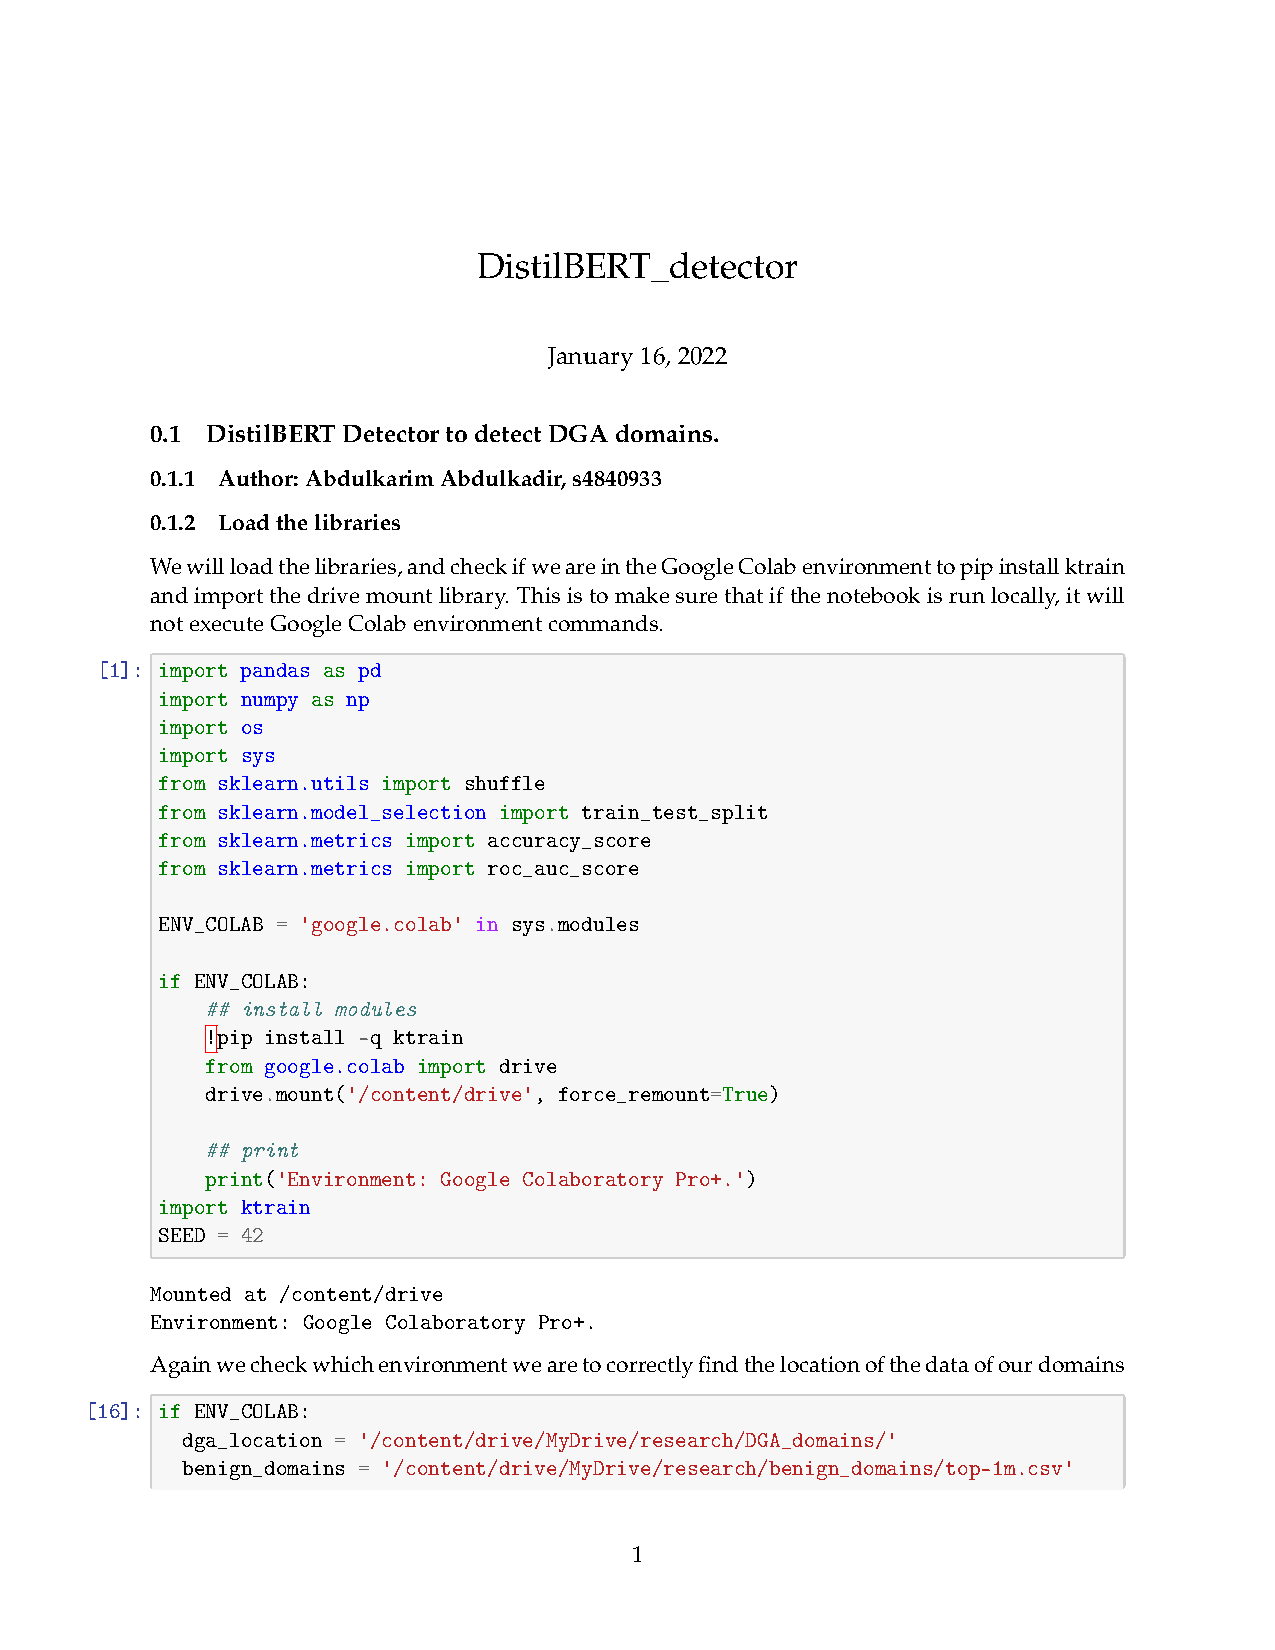
\includepdf[
%     pages=-, 
%     pagecommand={},
%     trim=0 2cm 0 2cm,
%     clip
% ]{DistilBERT_detector.pdf}